\documentclass{scrartcl}
\usepackage{amsmath,amsfonts,amsthm,bm,graphicx}
\usepackage{tikz,pgfplots}
\usepackage{listings}
\usepackage{stmaryrd}
\usepackage{xcolor}
\usepackage{rotating}
\usepackage{listings}
\usepackage{hyperref}

\pgfplotsset{width=15cm,compat=1.18}
\allowdisplaybreaks
\setlength{\parindent}{0pt}

\title{Assignment 6}
\subtitle{Angewandte Modellierung 25}
\author{Carl Colmant}
\date{\today}
\begin{document}
\maketitle
\newpage
\section*{Exercise 1. Data sets}
Ich habe mir ein Data set von Kaggle angeschaut welches schlaf betrachtet.(\href{https://www.kaggle.com/datasets/uom190346a/sleep-health-and-lifestyle-datasethttps://www.kaggle.com/datasets/mlomuscio/sleepstudypilot}{dataset}). Das Data set will heraus finden ob die Test Personen richtig einschätzen ob sie genug geschlafen haben. Hinzu wird noch die Existenz eines Smartphones in der nähe des Schalafplatzes getrackt und ob die Personen in den 30 Minuten vor dem Schlafengehen noch auf dem Smartphone waren.\\ 

\section*{Exercise 2. Word clouds}
Ich habe das Buch also sprach zarathhustra von Friedrich Nietzsche genommen und eine Wordcloud erstellt. Ich habe das Buch auf Project Gutenberg gefunden (\href{https://www.gutenberg.org/ebooks/7205https://www.gutenberg.org/ebooks/1998}{Project Gutenberg}). In diesem Buch legt Nietzsche seine theorie des Übermenschen und den alten Menschen dar. Ich habe so viele Füll wörter und Wörter die keine moralische bedeutung haben entfert und dann eine Wordcloud erstellt.\\
Dazu habe ich diesen Code benutzt:\\
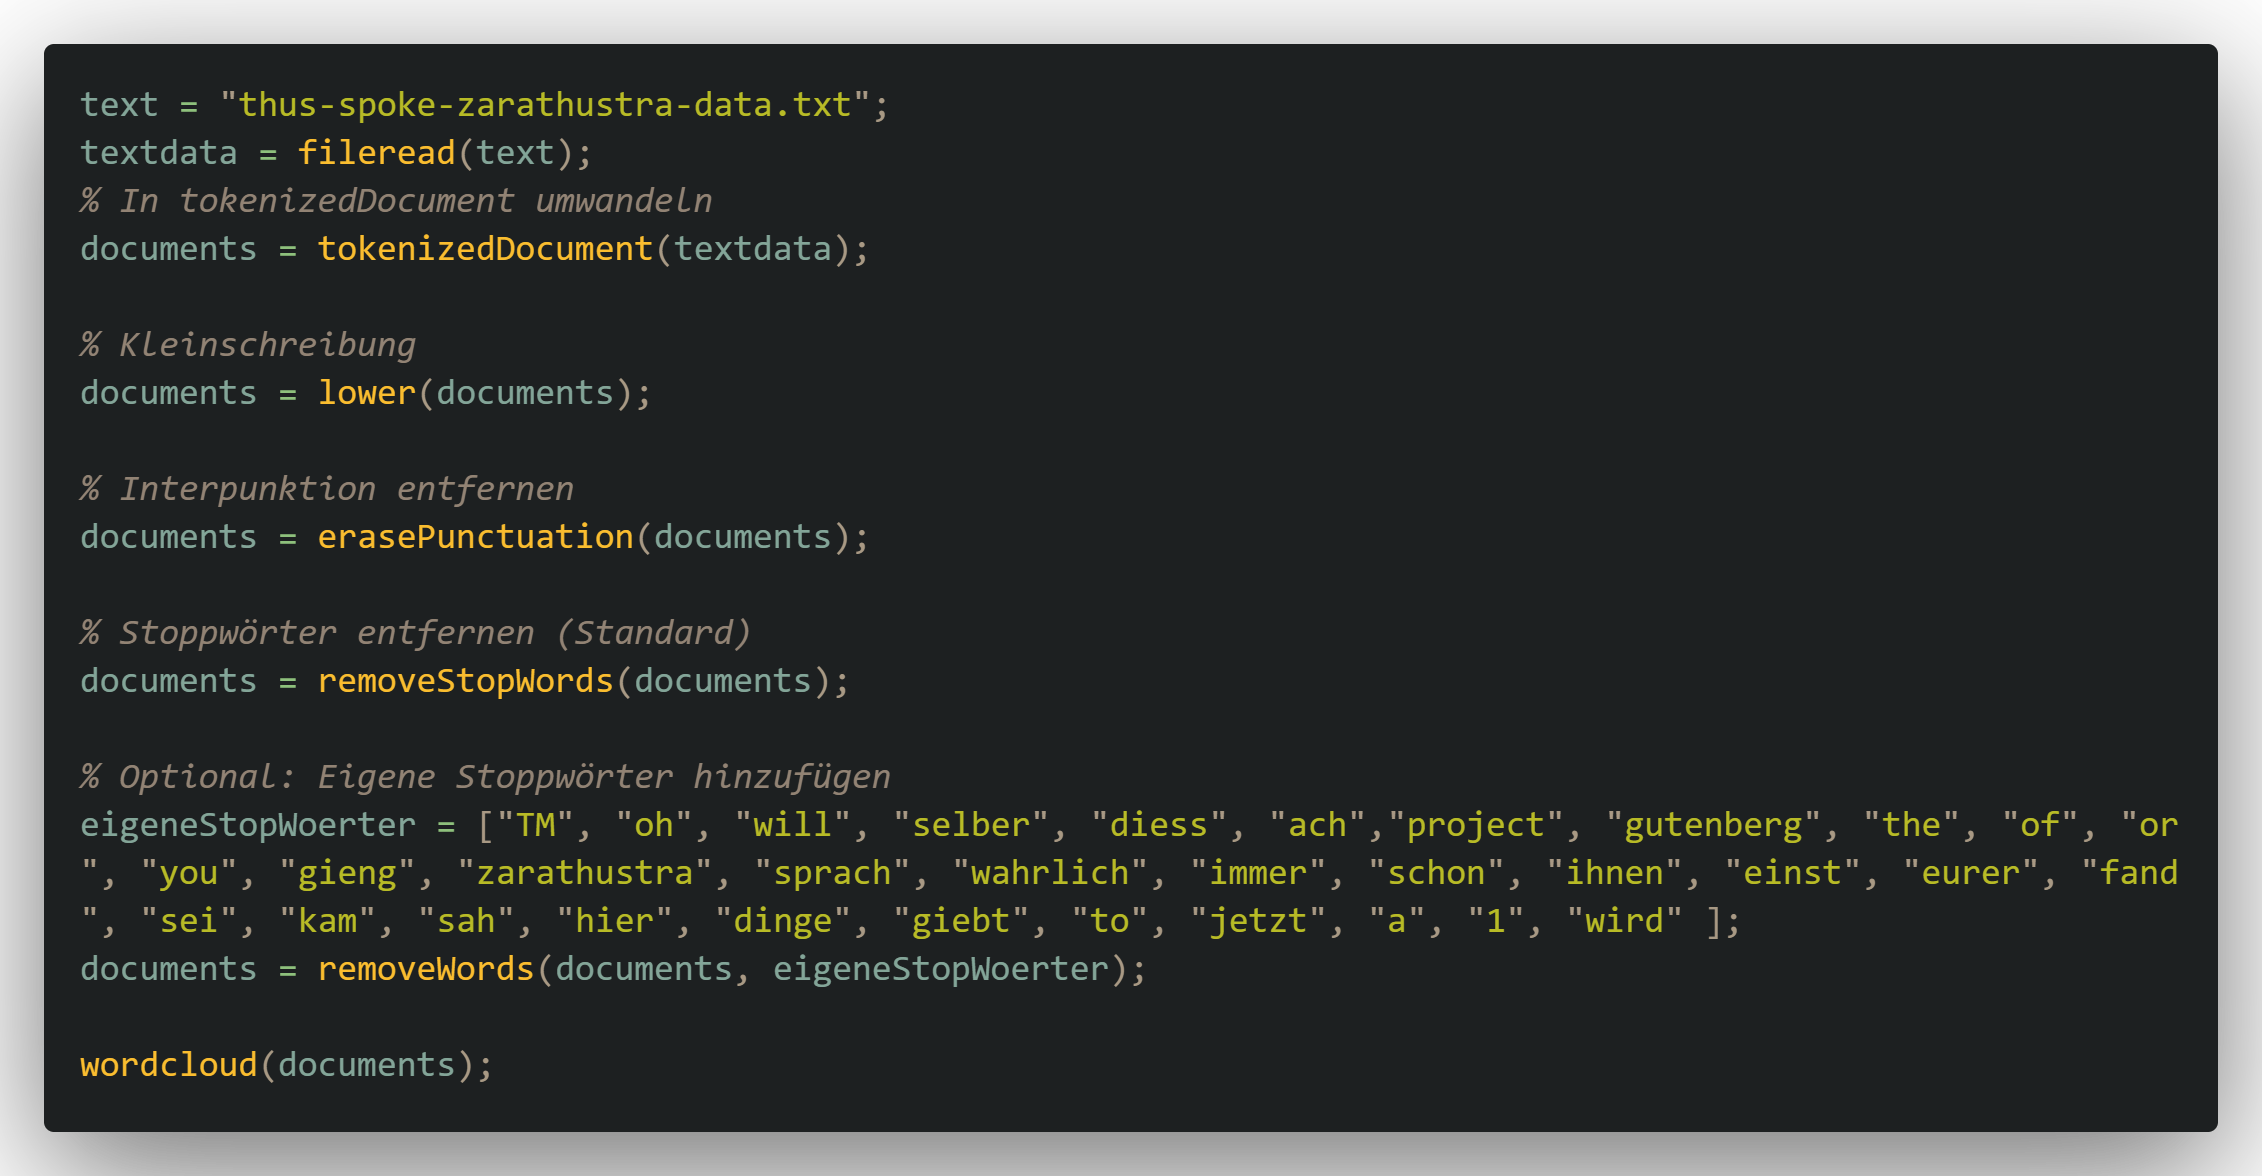
\includegraphics[scale=0.2]{code.png}\\
Das ist das Ergebnis:
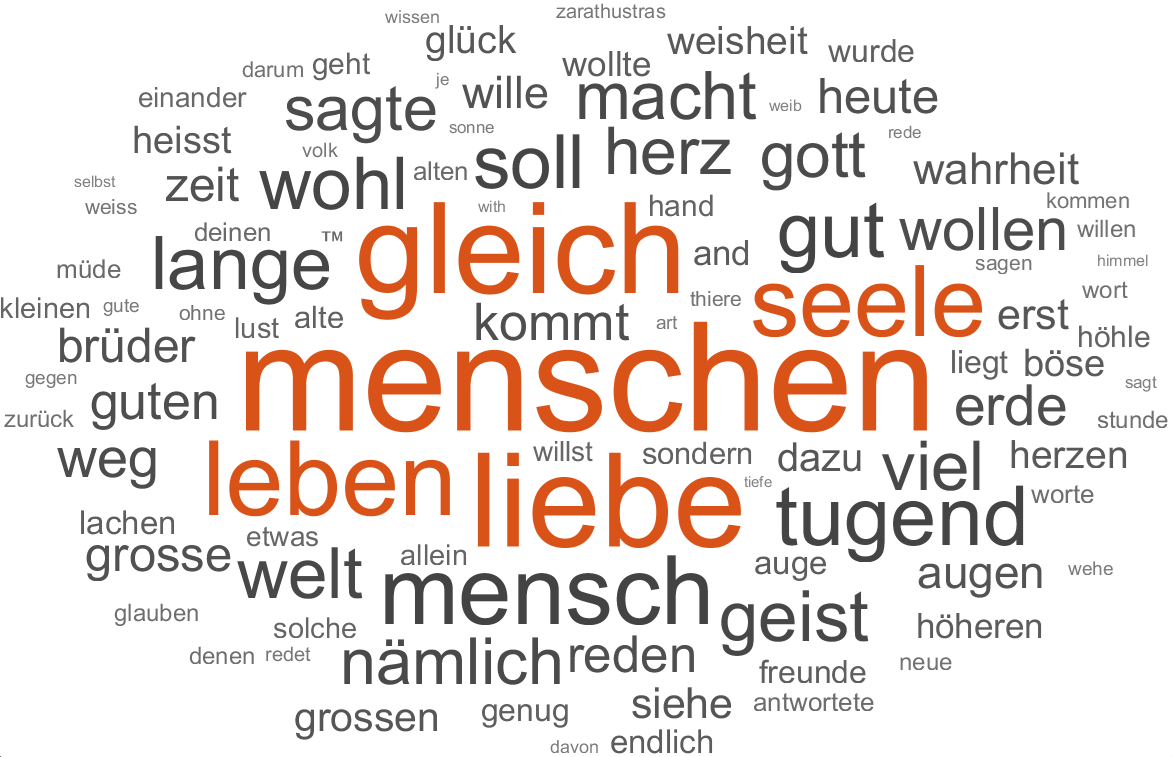
\includegraphics[scale=0.3]{wordcloud.png}\\
Man kann erkennen mit welchen Themen sich Nietzsche in diesem Buch beschäftigt hat. For allem der Seele und dem Geist also über natürlichen Dingen, aber auch über den Menschen und der Moral.\\


\section*{\href{https://github.com/7hands/Angewandte-Modellierung-25-Colmant}{Github}}
Wie immer sind alle meine benutzten Dateien auf meinem Github zu finden.




\end{document}